
\documentclass[unknownkeysallowed]{beamer}
\usetheme{Madrid}
\usepackage{subfig}
\usepackage{xcolor}
\usepackage{wrapfig}
\usepackage{braket}

\title{Dimensionality reduction with UMAP}
\subtitle{Advanced Data Mining seminar}
\author{Jakub Bartczuk}
\centering
\date{March 2020}
\begin{document}
\maketitle

\begin{frame}{Overview}
\tableofcontents[section,subsection]
\end{frame}

\begin{frame}{Teaser}
\framesubtitle{Reducing dimensionality of COIL20 Dataset}
\begin{figure}[ht]\centering\begin{minipage}[b]{0.45\linewidth}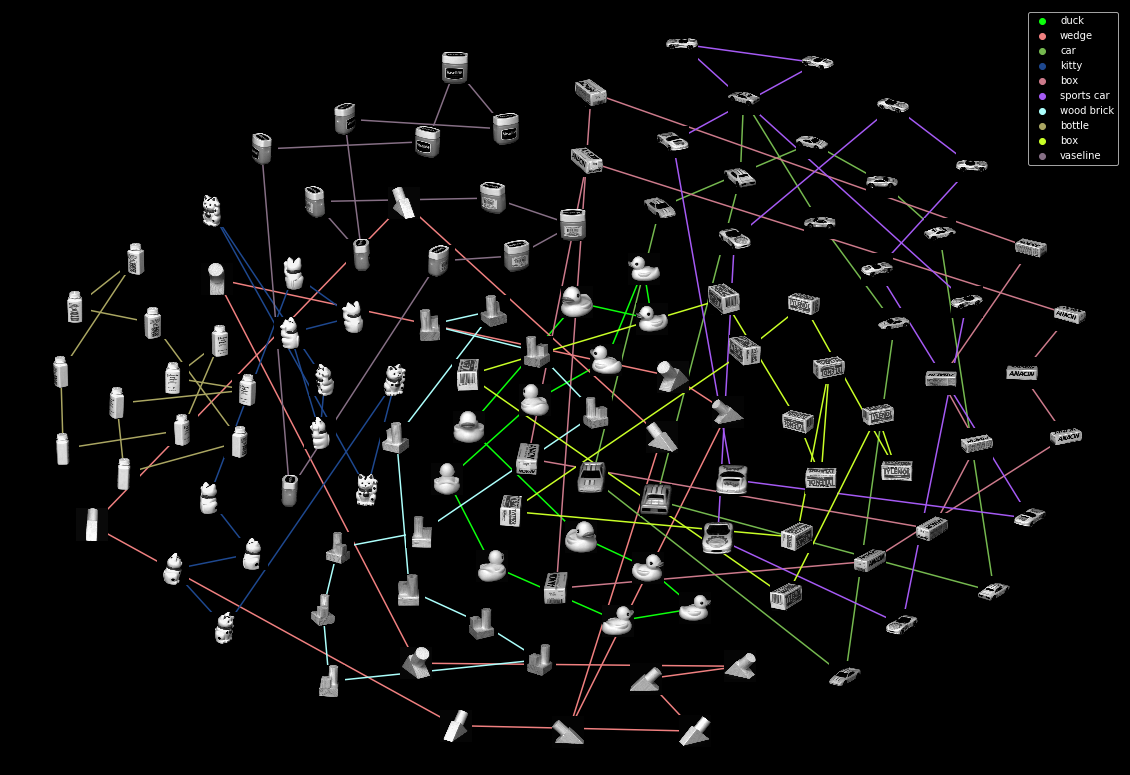
\includegraphics[width=\textwidth]{coil_tsne.png}\caption{tSNE}\label{fig:minipage1}\end{minipage}\quad\begin{minipage}[b]{0.45\linewidth}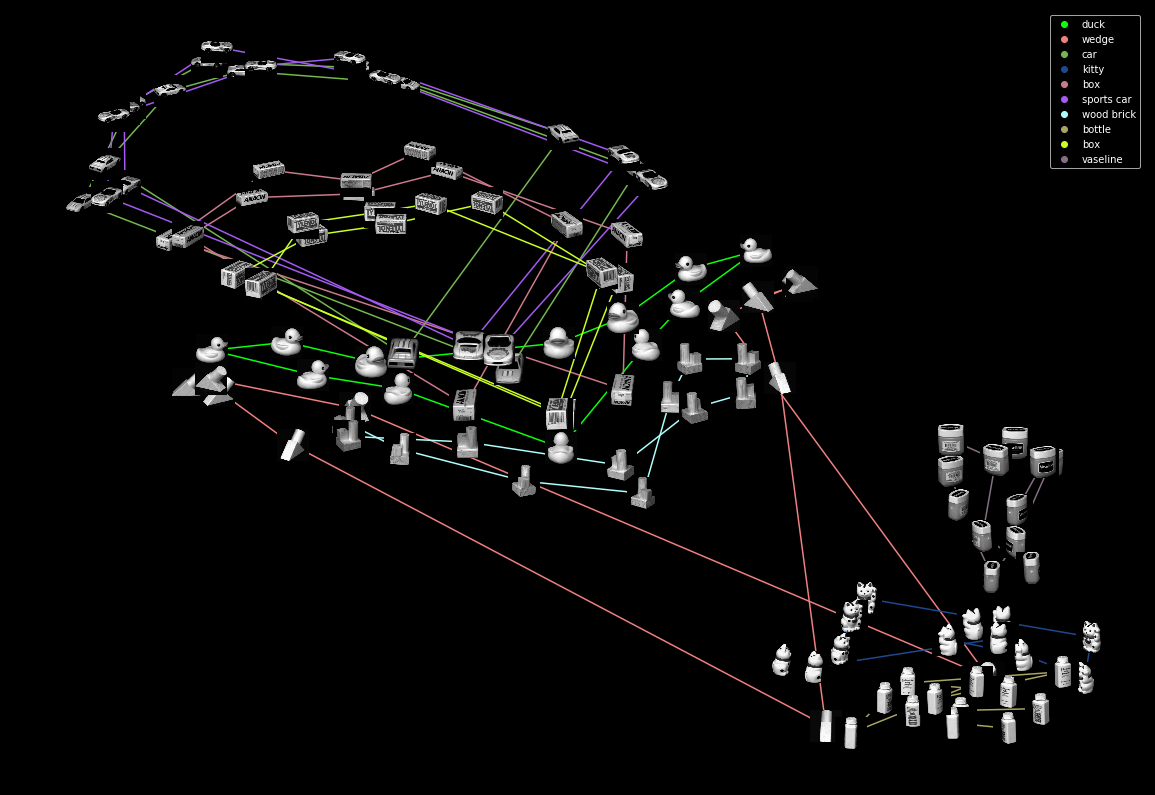
\includegraphics[width=\textwidth]{coil_umap.png}\caption{UMAP}\label{fig:minipage2}\end{minipage}\end{figure}
\end{frame}

\section{Manifold learning recap}
\begin{frame}{Manifold learning recap}

\begin{itemize}
\item We want to uncover lower-dimensional structure in high-dimensional space
\item Is the structure linear? If yes, use PCA
\item What to do if it is not linear?
\end{itemize}
\end{frame}
\begin{frame}{Manifold learning recap}



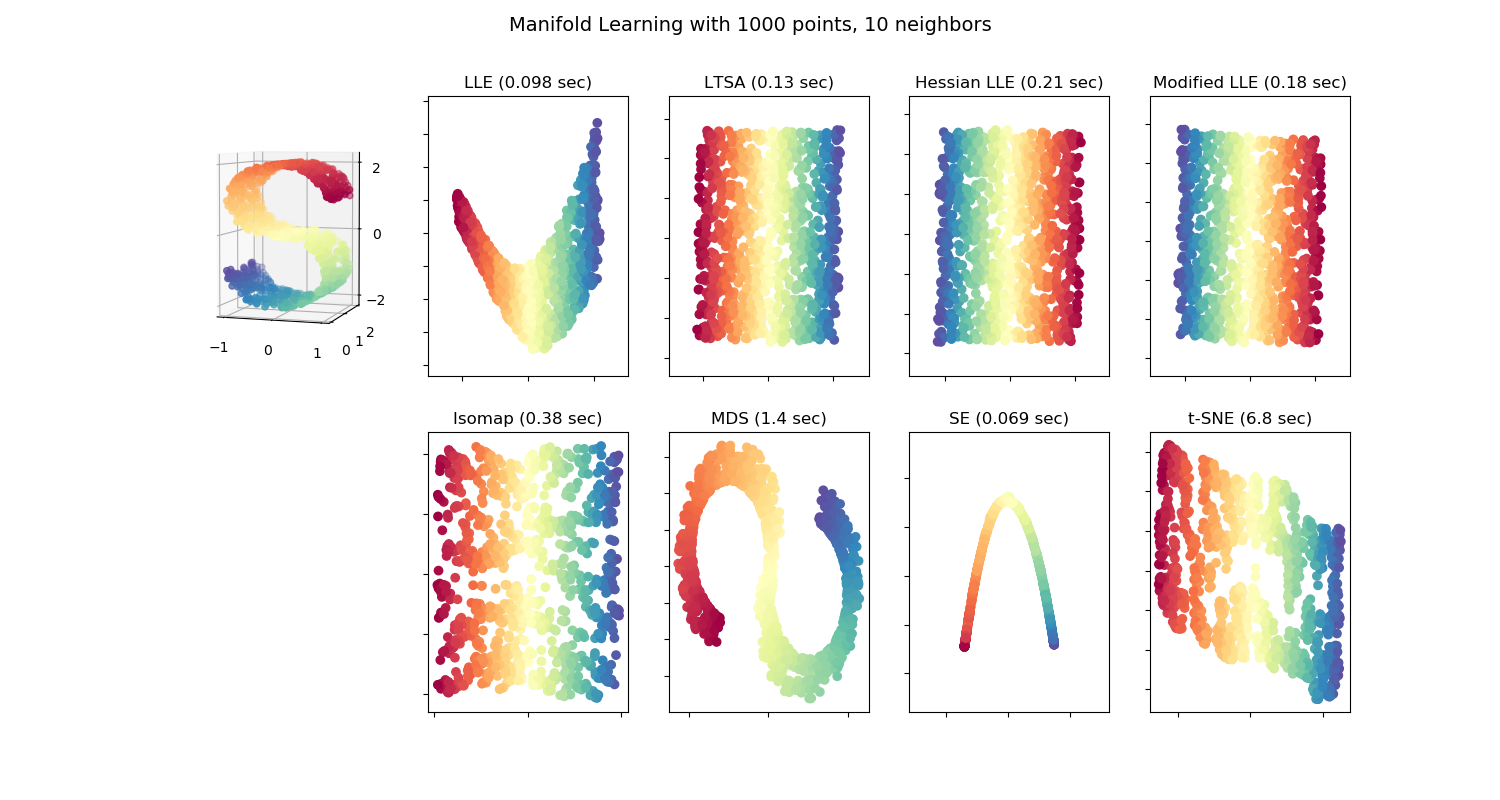
\includegraphics[width=\textwidth,height=0.8\textheight,keepaspectratio]{manifold_algorithms}

\end{frame}

\subsection{Multidimensional Scaling}
\begin{frame}{Classical Multidimensional Scaling}


$$D_{i,j} = \|x_i - x_j\|^2$$

Find $y$'s, $D'_{i,j} = \|y_i - y_j\|^2$ 

Such that $D' \approx D$

\end{frame}


\begin{frame}{Classical MDS properties}

\begin{itemize}
    \item easy to compute - decompose low-rank matrix from D
    \item fast - Euclidean distance matrix just couple of vectorized matrix computations
    \item treats all distortions alike
\end{itemize}



\begin{block}{What structure does MDS preserve?}
The last property basically means that we preserve local and global structure alike.

\begin{itemize}
    \item $x$'s are close - they are close in embedding.
    \item $x$'s are distant - they are equally distant in embedding.
\end{itemize}

\end{block}
\end{frame}
\subsection{Distances, graphs and matrix decomposition}

\begin{frame}{Distances, graphs and matrix decomposition}

\begin{block}{Local vs global structure}
We may not care about preserving exact large distances in embedding space as much as small distances

\textcolor{red}{Idea}: Calculate distance along the set 'spanned' by datapoints
\end{block}

\begin{block}{Manifold hypothesis}
The data lies in lower-dimensional, possibly nonlinear space which is embedded in ambient space
\end{block}



\end{frame}

\begin{frame}{MDS breakdown}


\begin{enumerate}
   \item estimate distances between some pairs of close points
   \item make graph $(X, E)$ with edges weighted by distance
   \item define $D$ as distance from graph
   \item decompose matrix that represents the graph
\end{enumerate}{}

\begin{block}{Getting manifold learning algorithms from schematic}

\begin{itemize}
    \item Setting $E = \{((x_i, x_j), \|x_i - x_j\|^2) | x_i, x_j \in X \}$ (complete graph) we get classical MDS
    \item Modifying steps 1-3 will get us Isomap, Hessian Eigenmaps
    \item tSNE and UMAP will change step 4
\end{itemize}
\end{block}



\end{frame}

\section{Stochastic Neighbor Embedding}
\begin{frame}{Stochastic Neighbor Embedding}

Idea: embed into lower-dimensional space, preserve distance statistics

$$q_{j|i} = \frac{\textcolor{blue}{f}(\|y_i - y_j\|)}{\sum_{k \neq j}\textcolor{blue}{f}(\|y_i - y_k\|)}, p_{j|i} = \frac{exp(-\|x_i - x_j\|^2 / \textcolor{red}{\sigma^2_i})}{\sum_{k \neq j}exp(-\|x_i - x_k\|^2/\textcolor{red}{\sigma^2_i})}$$

$$KL(p, q) = \sum_{i, j} p_{j|i} log\frac{p_{j|i}}{q_{j|i}}$$

\begin{block}{Notes}
Choice of $\textcolor{blue}{f}$ determines algorithm:
\begin{itemize}
    \item $\textcolor{blue}{f(x) = exp(-x^2)}$ - original SNE
    \item $\textcolor{blue}{f(x) = (1 + x^2)^{-1}}$ - tSNE (note this is density of Cauchy distribution up to a constant)
\end{itemize}
\end{block}
\end{frame}

\begin{frame}{Stochastic Neighbor Embedding}

\begin{block}{Perplexity}
\textcolor{red}{$\sigma_i$} gives rise to perplexity $P_i = 2^{H(p_i)}$ which controls effective neighborhood size at $x_i$.
\end{block}

\begin{block}{Algorithm}
\begin{itemize}
	\item for each $x_i$ find $\sigma_i$ that matches given perplexity
    \item initialize $y_i$ randomly
    \item minimize KL with gradient descent w.r.t. $y_i$
\end{itemize}
\end{block}

\end{frame}


\begin{frame}{Problems with SNE: Crowding problem}

\begin{columns}[onlytextwidth]
\begin{column}[T]{.48\textwidth}
\begin{itemize}
	\item 'more room' for intermediate distances in higher dimensions

	\item pairs of points will tend to have similar distance (\textcolor{red}{remember curse of dimensionality for kNN})
	\item harder to embed them faithfully into lower dimensional space

\end{itemize}
\end{column}

\begin{column}[T]{.48\textwidth}
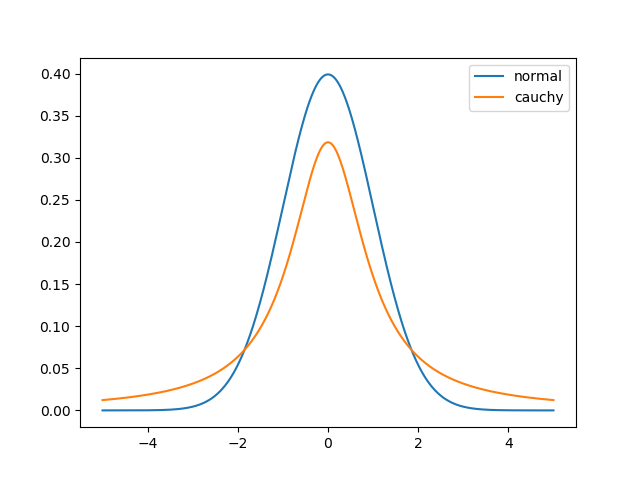
\includegraphics[width=\textwidth]{long_tail.png}
\end{column}
\end{columns}

\begin{itemize}
\item somewhat fixed by using t Distribution which has longer tails (not so concentrated about maximum).

This problem is not specific to tSNE - it relates to the fact that data may not be sampled uniformly from manifold
\end{itemize}

\end{frame}

\section{UMAP}


\begin{frame}{ELI5 UMAP}

\begin{flushleft}
Recall UMAP means \textbf{Uniform} Manifold Approximation and Projection
\end{flushleft}

\end{frame}

\begin{frame}{UMAP vs tSNE}
\begin{tabular}{c|c|c}
& UMAP & tSNE\\
\hline
Initialization & Embedding from graph matrix decomposition & Random Gaussian \\
\hline
Optimization & SGD + negative sampling & Gradient Descent \\
\end{tabular}
\end{frame}

\begin{frame}{UMAP vs tSNE}

{\scalebox{1.4}{
\begin{tabular}{c|c|c}
 & UMAP & tSNE \\
 \hline
 $p_{i|j}$ & $exp(- \frac{d(x_i, x_j) - \textcolor{green}{\rho_i}}{\textcolor{green}{\sigma_i}})$ & $\frac{exp(-\|x_i - x_j\|^2 / \textcolor{red}{s^2_i})}{\sum_{k \neq j}exp(-\|x_i - x_k\|^2/\textcolor{red}{\sigma^2_i})}$ \\
 \hline
 $q_{i|j}$ & $(1 + a\|y_i - y_j\|^{2b}))^{-1}$ & $\frac{(1 + (\|y_i - y_j\|^2))^{-1}}{\sum_{k \neq j}(1 + (\|y_i - y_k\|^2))^{-1}}$ \\
 \hline
 {\small Loss} & {\tiny H(q, p) = H(p) + KL(q, p)} & {\tiny KL(q, p)}
\end{tabular}
}
}
\begin{block}{Where do $\textcolor{green}{\rho_i}, \textcolor{green}{\sigma_i}$ come from?}
Enter Riemannian structure
\end{block}
\end{frame}



\subsection{Topological and geometrical preliminaries}

\begin{frame}{Riemannian structure}

Remember we want to calculate distance \textbf{along the manifold} 

Curve length on manifold $\to$ distance on manifold

\begin{block}{Curve length in Euclidean space}

$L_\gamma = \int_{0}^{1} \|\gamma'(t)\| dt =  \int_{0}^{1} \sqrt{\braket{\gamma'(t) | \gamma'(t)}} dt$

\end{block}

\textit{Riemannian space} has local inner product

Estimate Riemannian structure with finite samples - set it constant on neighborhoods

Scale neighborhoods so that we have evenly spaced samples

\begin{alertblock}{Problem}
We get incompatible local structures
\end{alertblock}
\end{frame}



\begin{frame}{Topological preliminaries}
Topology is the study of structures that are \textit{invariant under continuous transformations}

Here we're interested in spaces that can be expressed from simpler spaces - like polyhedrons

\end{frame}


\begin{frame}{Topological preliminaries}

\begin{columns}[T]
\begin{column}{0.5\linewidth}

\begin{block}{Simplex}
A $d$-dimensional simplex is a set $S \subset \mathbb{R}^n$ such that there are $d$ linearly independent points $S = conv(d)$ 

\end{block}

\begin{block}{Simplicial complex}
A set $C$ of simplexes such that if $s, s' \in C \implies s \cap s' \in C$ 
\end{block}
\end{column}
\begin{column}{0.5\linewidth}
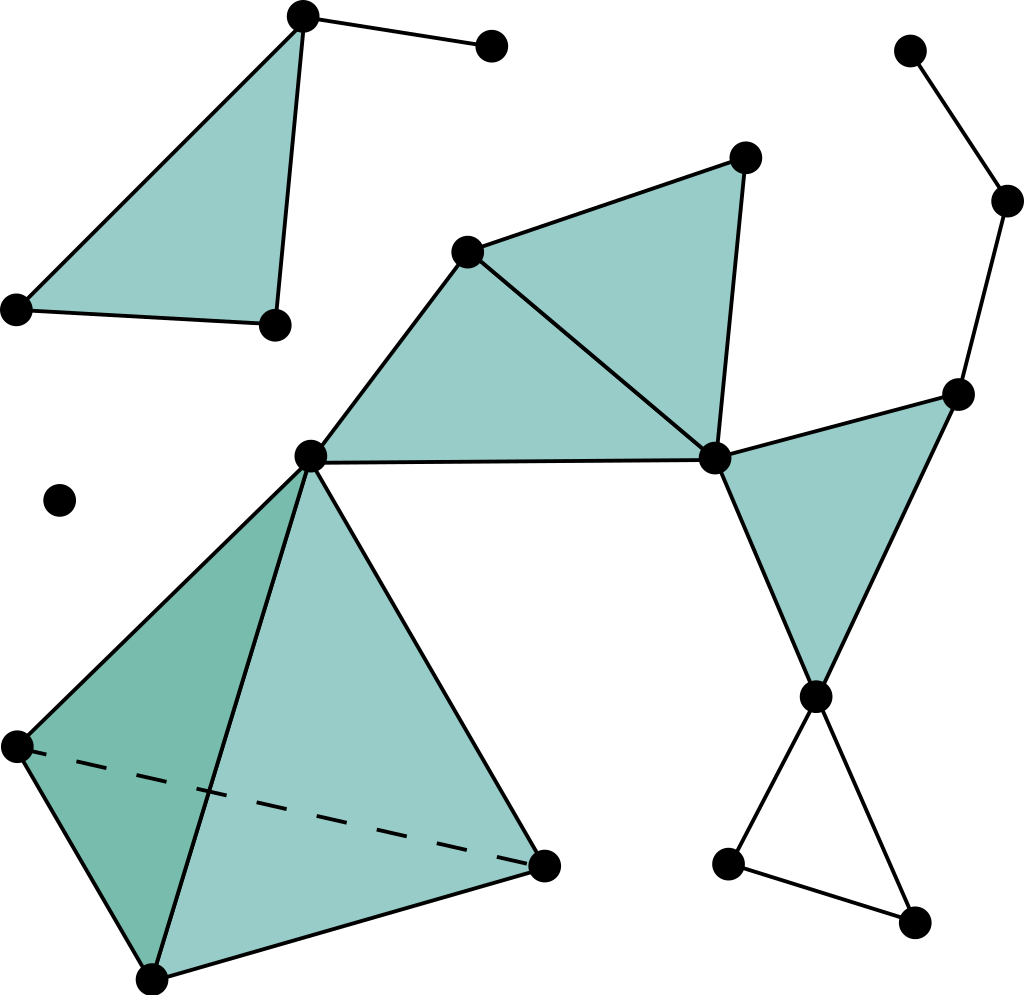
\includegraphics[width=\textwidth,height=0.5\textheight,right]{Simplicial_complex_example.svg.png}

\end{column}
\end{columns}
\end{frame}



\begin{frame}{Topology}

\begin{block}{Nerve theorem}

\end{block}
\end{frame}

\begin{frame}{Global structure from local structures}

\end{frame}

\section{Experiments}

\begin{frame}{Experiments}

\end{frame}

\section{Practicalities}
\begin{frame}{Algorithmic considerations}

\end{frame}

\begin{frame}{Python implementations}

	\begin{block}{tSNE and other algorithms}
		\begin{itemize}
			\item scikit-learn implements tSNE, MDS, Isomap, Hessian Eigenmaps, Locally Linear Embedding
			\item faster implementations available in \texttt{megaman} package
		\end{itemize}
	\end{block}
	
	\begin{block}{UMAP}
		\begin{itemize}
			\item original author's package (\texttt{pip install umap-learn})
			\item GPU accelerated NVidia \texttt{rapids (cuML)} 
		\end{itemize}
	\end{block}
\end{frame}
\end{document}
